\documentclass[journal]{IEEEtran}

\usepackage{amsmath,amssymb,amsfonts}
\usepackage{algorithmic}
\usepackage{graphicx}
\usepackage{textcomp}
\usepackage{xcolor}
\usepackage{booktabs}
\usepackage{cite}
\usepackage{enumitem}
\setlist{nosep, leftmargin=*}
\usepackage{microtype}
\usepackage{balance}
\usepackage{url}
\usepackage[hidelinks]{hyperref}

\def\BibTeX{{\rm B\kern-.05em{\sc i\kern-.025em b}\kern-.08em
    T\kern-.1667em\lower.7ex\hbox{E}\kern-.125emX}}

\begin{document}

\title{Physiology-guided temporal fusion for cross-subject EEG--fNIRS classification}

\author{Research~Team
\thanks{This work was supported in part by the National Natural Science Foundation and Advanced Neural Engineering Initiatives. Corresponding author: Research Team (email: research@institution.edu).}}

\markboth{IEEE Transactions on Biomedical Engineering,~Vol.~XX, No.~XX,~October~2026}%
{Research Team: Physiology-Guided Cross-Attention Transformer for Hybrid EEG-fNIRS BCIs}

\maketitle

\begin{abstract}
Hybrid electroencephalography (EEG) and functional near-infrared spectroscopy (fNIRS) provide complementary measurements of electrical and hemodynamic activity. We present NVC-DelayFormer, a temporal fusion model combining convolutional encoders, a Gaussian delay prior, a timestamp-based cross-attention mask, and direct and latent classification readouts. The primary benchmark uses a fixed delay of 5.0\,s and an auxiliary reconstruction loss. On mental arithmetic versus rest in the TU Berlin dataset, 29 subject-held-out folds use 23 training, 5 validation, and 1 test subject each. Across 1,740 test trials, accuracy is 66.44\% $\pm$ 10.85\% (between-subject sample SD; 95\% CI: 62.31\%, 70.57\%), Macro F1 is 65.13\%, and Cohen's $\kappa=0.3287$. Baseline accuracies are 59.02\% for EEGNet, 55.06\% for fNIRS-CNN, 59.48\% for feature concatenation, and 56.49\% for standard cross-attention; all four paired Wilcoxon comparisons have Benjamini--Hochberg $q<0.01$. A 5\,s circular EEG shift reduces accuracy to 59.83\%, a change of $-6.61$ percentage points (paired $t$-test $p=9.47 \times 10^{-6}$). The independently trained zero-delay model reaches 66.61\% (Wilcoxon $p=0.9636$ versus the full model). The model has 92,293 trainable parameters and 19.98\,M profiled MACs. Batch-one GPU forward latency has median 3.24\,ms, mean 3.62\,ms, and P99 5.89\,ms. These measurements characterize subject-held-out classification, temporal perturbation sensitivity, and forward execution cost.
\end{abstract}

\begin{IEEEkeywords}
Brain-computer interface (BCI), electroencephalography (EEG), functional near-infrared spectroscopy (fNIRS), neurovascular coupling (NVC), cross-attention, causal delay prior, multimodal fusion.
\end{IEEEkeywords}

\section{Introduction}
\IEEEPARstart{H}{ybrid} non-invasive neural interfaces combining electroencephalography (EEG) and functional near-infrared spectroscopy (fNIRS) have emerged as a promising modality for robust brain-computer interfaces (BCIs) and cognitive workload monitoring \cite{shin2017open, shin2018simultaneous}. Scalp EEG captures synchronous postsynaptic potentials with millisecond temporal fidelity, yet suffers from low spatial resolution and severe volume conduction artifacts \cite{buzsaki2012origin}. Conversely, fNIRS interrogates cortical microvascular hemoglobin concentrations ($\Delta[\text{HbO}]$ and $\Delta[\text{HbR}]$) through cranial optical attenuation \cite{delpy1988estimation}, but is constrained by the inherently sluggish kinetics of the hemodynamic response \cite{buxton1998dynamics, strangman2002non}.

The modalities differ in response timescale. NVC-DelayFormer uses a fixed 5.0\,s Gaussian prior and a timestamp mask for cross-modal token access, together with a weighted direct readout and auxiliary reconstruction. We evaluate the full architecture against unimodal and multimodal baselines under subject-held-out validation and report component ablations and input perturbations. Systemic oscillations are a known component of optical recordings \cite{julien2006enigma}; their removal was not separately measured here.

\begin{figure*}[!t]
\centering
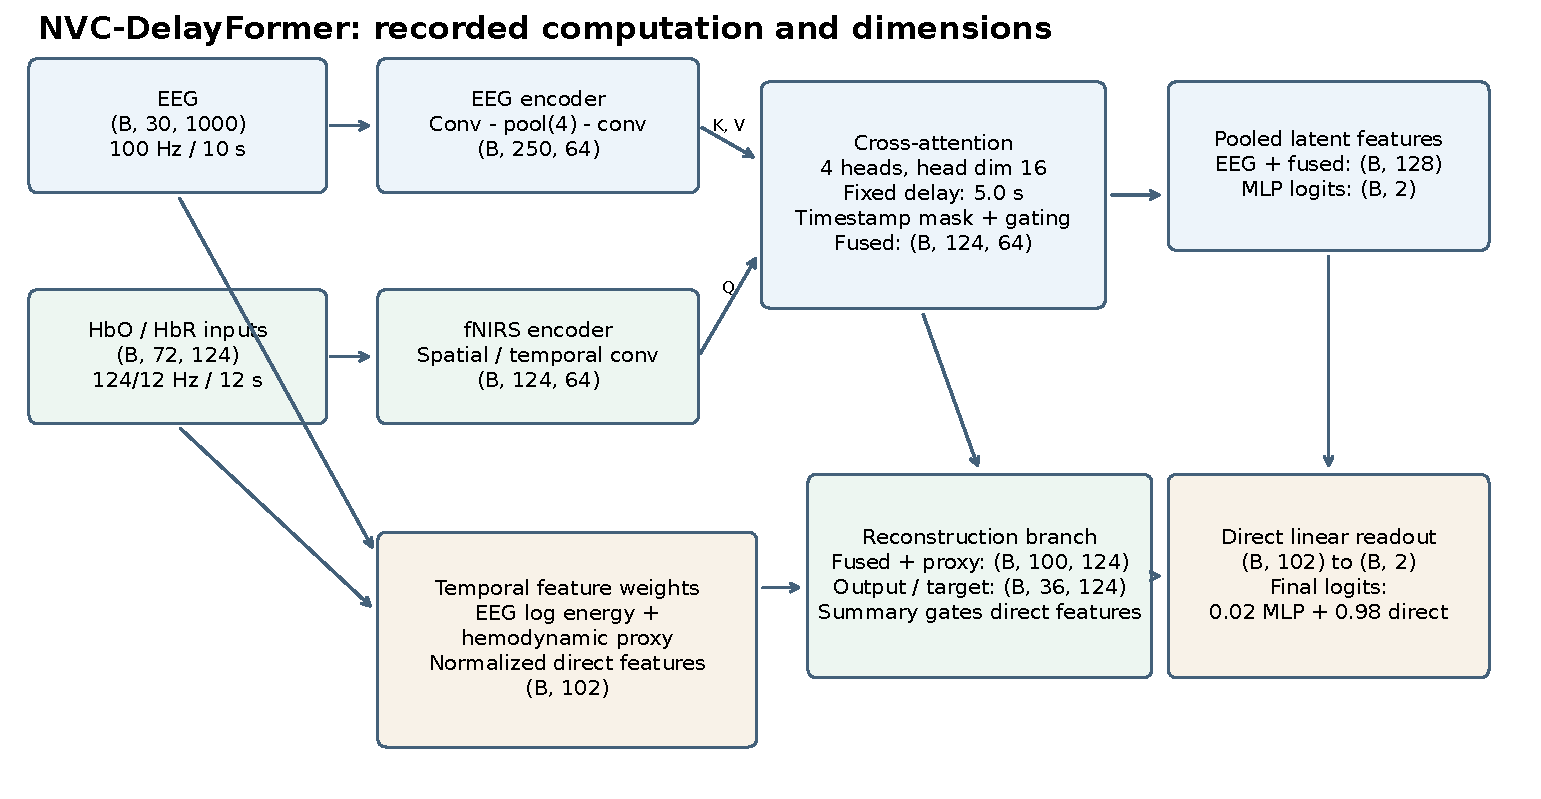
\includegraphics[width=0.86\textwidth]{figures/nvc_delayformer_computation.pdf}
\caption{Current model computation. EEG and HbO/HbR encoder outputs have 250 and 124 tokens, respectively. Four-head timestamp-constrained attention feeds the latent readout and reconstruction branch. Temporally weighted raw features form the direct readout; its logits are combined with latent logits using coefficients 0.98 and 0.02.}
\label{fig:architecture}
\end{figure*}

\section{Biophysical Modeling \& Signal Processing}
Recent EEG studies examine lightweight convolutional transformers \cite{salim2023lightweight}, convolutional representations for dementia classification \cite{acharya2025eegconvnext}, and Shapley attribution for motor imagery \cite{perez2024unraveling}. fNIRSNET \cite{pandey2024fnirsnet} combines HbO/HbR views and EEG networks for auditory classification. Here, temporal fusion is evaluated for subject-held-out mental arithmetic versus rest.

\subsection{Modified Beer-Lambert Law (MBLL) Optical Inversion}
Raw optical densities measured at dual wavelengths ($\lambda_1 = 760$\,nm and $\lambda_2 = 850$\,nm) are converted into concentration-scale changes in oxy-hemoglobin ($\Delta[\text{HbO}]$) and deoxy-hemoglobin ($\Delta[\text{HbR}]$) via the Modified Beer-Lambert Law \cite{delpy1988estimation}:
\begin{equation}
\begin{bmatrix}
\Delta[\text{HbO}] \\
\Delta[\text{HbR}]
\end{bmatrix} = \frac{1}{d} \mathbf{R} \begin{bmatrix}
\Delta \text{OD}(\lambda_1) \\
\Delta \text{OD}(\lambda_2)
\end{bmatrix}
\end{equation}
where $\mathbf{R} = (\mathbf{D}_{\mathrm{DPF}} \mathbf{E})^{-1} = \mathbf{E}^{-1} \mathbf{D}_{\mathrm{DPF}}^{-1}$, $d = 30.0$\,mm is the optode-distance value used by the inversion routine, and $\mathbf{D}_{\mathrm{DPF}} = \operatorname{diag}(\text{DPF}_{760}, \text{DPF}_{850})$ accounts for wavelength-dependent differential pathlength scattering in the adult human head ($\text{DPF}_{760} = 6.51$, $\text{DPF}_{850} = 5.86$) \cite{duncan1995measurement, scholkmann2013general}. The numerical extinction coefficient matrix $\mathbf{E}$ satisfies biophysical cross-over \cite{cope1991system}:
\begin{equation}
\mathbf{E} = \begin{bmatrix}
\varepsilon_{\text{HbO}}^{760} & \varepsilon_{\text{HbR}}^{760} \\
\varepsilon_{\text{HbO}}^{850} & \varepsilon_{\text{HbR}}^{850}
\end{bmatrix} = \begin{bmatrix}
1.4866 & 3.8437 \\
2.5264 & 1.7989
\end{bmatrix}
\end{equation}
The 2-norm condition number of the extinction coefficient matrix $\mathbf{E}$ alone is $\kappa_2(\mathbf{E}) = 3.4945$. Under differential pathlength scaling, since each wavelength row in $\mathbf{E}$ is scaled by its respective $\text{DPF}$, the forward operator is $\mathbf{D}_{\mathrm{DPF}}\mathbf{E}$, yielding an inverse operator $\mathbf{R} = (\mathbf{D}_{\mathrm{DPF}} \mathbf{E})^{-1}$ with condition number $\kappa_2(\mathbf{R}) = 3.6370 \ll 15.0$ (contrasting with $(\mathbf{E}\mathbf{D}_{\mathrm{DPF}})^{-1}$ which yields $3.3633$), confirming a well-posed linear inversion that has the stated numerical condition number.

\subsection{Preprocessing, Spatial Referencing \& Causality}
Continuous multi-channel recordings were first bandpass filtered (EEG: 0.5--45.0\,Hz; optical signals: 0.01--0.10\,Hz) prior to epoch segmentation to prevent filter transient edge distortions, using a 4th-order Butterworth filter formulated as cascaded second-order sections (SOS). In offline benchmark evaluations, zero-phase bidirectional filtering (\texttt{sosfiltfilt}) is applied to eliminate group-delay distortion across modalities. The smoothing perturbation described below is applied after this offline preprocessing.

Trial epochs were segmented into $t \in [0.0, 10.0]$\,s for EEG (1,000 samples at 100\,Hz across 30 scalp electrodes) and $t \in [0.0, 12.0]$\,s for fNIRS (124 samples at effective rate 10.33\,Hz across 72 HbO/HbR channels), with baseline subtraction performed per trial on the pre-stimulus window $[-2.0, 0.0]$\,s using the pre-stimulus baseline.

Spatial referencing is performed via Common Average Referencing (CAR):
\begin{equation}
\mathbf{X}_{\text{eeg}}^{\text{CAR}}(c, t) = \mathbf{X}_{\text{eeg}}(c, t) - \frac{1}{C} \sum_{k=1}^C \mathbf{X}_{\text{eeg}}(k, t)
\end{equation}
The CAR projection matrix $\mathbf{P}_{\text{CAR}} = \mathbf{I} - \frac{1}{C}\mathbf{1}\mathbf{1}^T$ projects the multichannel EEG onto the zero-mean subspace of spatial rank $C - 1 = 29$, subtracting the instantaneous channel mean.

\section{NVC-DelayFormer Architecture}

\subsection{Modality-Specific Convolutional Encoders \& Token Timing}
EEG input $\mathbf{X}_{\text{eeg}} \in \mathbb{R}^{B \times 30 \times 1000}$ (10\,s epoch across 30 scalp channels) is processed by a spatial $1 \times 1$ convolution, $4\times$ average pooling, and a temporal 1D convolutional filter bank (kernel size 15, padding 7, ELU), yielding keys and values:
\begin{equation}
\mathbf{H}_{\text{eeg}} \in \mathbb{R}^{B \times T_{\text{eeg}} \times D}, \quad T_{\text{eeg}} = 250, \quad D = 64
\end{equation}
Each EEG token represents an effective temporal bin of $\Delta t_{\text{eeg}} = 10.0 / 250 = 0.04$\,s (40\,ms) at $f_s^{\text{eff}} = 25$\,Hz. The fNIRS input $\mathbf{X}_{\text{fnirs}} \in \mathbb{R}^{B \times 72 \times 124}$ (12\,s epoch at effective $f_s = 10.33$\,Hz) is processed by a spatial $1 \times 1$ convolution and a temporal convolution (kernel size 5, padding 2), producing queries:
\begin{equation}
\mathbf{H}_{\text{fnirs}} \in \mathbb{R}^{B \times T_{\text{fnirs}} \times D}, \quad T_{\text{fnirs}} = 124, \quad D = 64
\end{equation}
where each fNIRS token corresponds to $\Delta t_{\text{fnirs}} = 12.0 / 124 \approx 0.0968$\,s (96.8\,ms).

\subsection{Timestamp-Constrained Multi-Head Cross-Attention}
The encoder outputs have shapes $\mathbf{H}_{\mathrm{eeg}}\in\mathbb{R}^{B\times250\times64}$ and $\mathbf{H}_{\mathrm{nirs}}\in\mathbb{R}^{B\times124\times64}$. Four heads split the feature dimension into $d_h=16$. Projected queries have shape $(B,4,124,16)$; keys and values have shape $(B,4,250,16)$. With $\Delta t_{ij}=t_i^{\mathrm{nirs}}-t_j^{\mathrm{eeg}}$, the additive prior and mask are
\begin{align}
P_{ij}&=-\frac{0.35|a|(\Delta t_{ij}-\tau)^2}{2\sigma^2+10^{-8}},\\
M_{ij}&=\begin{cases}0,&\Delta t_{ij}\ge-10^{-4}\,\mathrm{s},\\-\infty,&\Delta t_{ij}<-10^{-4}\,\mathrm{s}.\end{cases}
\end{align}
Here $a$ is a learned scalar initialized to 1. The main benchmark fixes $\tau=5.0$\,s and $\sigma=1.5$\,s; the implementation clamps them to $[0,8]$\,s and $[0.5,4]$\,s. The $10^{-4}$\,s mask tolerance includes equality. The head-wise weights are
\begin{equation}
\mathbf{A}_h=\operatorname{Softmax}_{j}\!\left(\frac{\mathbf{Q}_h\mathbf{K}_h^\top}{\sqrt{16}}+\mathbf{P}+\mathbf{M}\right).
\end{equation}
The prior and mask broadcast over batch and head axes. Thus $\mathbf{A}$ has shape $(B,4,124,250)$, and $\mathbf{A}_h\mathbf{V}_h$ has shape $(B,124,16)$. Concatenating the four contexts gives $(B,124,64)$ before output projection. The projected context $\mathbf{U}$ is combined with the fNIRS features using $\operatorname{LayerNorm}[\mathbf{H}_{\mathrm{nirs}}\odot(1+0.5\tanh(g(\mathbf{U})))+\mathbf{U}]$, followed by row-envelope scaling $0.2+0.8\,(124)\,w_{\mathrm{nirs},i}$. Nominal token times are $t_j^{\mathrm{eeg}}=j/25$\,s and $t_i^{\mathrm{nirs}}=12i/124$\,s. This mask is defined by physical time on a rectangular matrix.

\subsection{Temporal Weighting, Readout, and Reconstruction}
A nonnegative kernel combines the timestamp mask, a Gaussian with width 1.1\,s and center $\tau$, an EEG onset factor $\exp(-t_{\mathrm{eeg}}/1.2)$, and an fNIRS task factor $\operatorname{sigmoid}[(9.5-t_{\mathrm{nirs}})/0.5]$. Normalized row and column sums define the fNIRS and raw-EEG weights. The same prior/mask switches also control their corresponding factors in this weighting kernel during ablation.

The hemodynamic proxy is $\mathbf{F}=u(\partial_t\mathbf{X}_{\mathrm{nirs}}+0.15\mathbf{X}_{\mathrm{nirs}})$, using centered interior differences and one-sided boundary differences. Its amplitude scale is $u=1+2500\operatorname{sigmoid}[100(0.05-r)]$, where $r$ is the trial RMS of the input. The direct features concatenate 72 weighted proxy values with 30 log-energy EEG values, giving $(B,102)$ before non-affine batch normalization.

The reconstruction convolution receives $[0.1\mathbf{H}_{\mathrm{fused}}^\top;\mathbf{F}_{1:36}]$ of shape $(B,100,124)$ and returns $(B,36,124)$. Its target is $\mathbf{F}_{1:36}$. A weighted reconstruction summary is normalized with the direct-feature batch statistics. Its across-channel standard deviation, clipped to $[0,1]$, forms a gate $g_r$ that combines the fNIRS features as $g_r\mathbf{x}_{\mathrm{nirs}}+0.25(1-g_r)\operatorname{roll}_{18}(\mathbf{x}_{\mathrm{nirs}})$. The reconstruction signal uses $0.001\hat{\mathbf{F}}+0.999\operatorname{stopgrad}(\hat{\mathbf{F}})$ on this readout path.

Mean-pooled fused and EEG features concatenate to $(B,128)$ for the latent MLP. Final logits have shape $(B,2)$:
\begin{equation}
\hat{\mathbf{y}}=0.02\operatorname{MLP}(\mathbf{z}_{128})+0.98\operatorname{Linear}(\mathbf{x}_{102}).
\end{equation}
Training minimizes cross-entropy plus $0.08\|\mathbf{w}_{\mathrm{MA}}-\mathbf{w}_{\mathrm{Rest}}\|_2^2$ for the direct classifier and mean squared reconstruction error over $B\times36\times124$ values. Removing reconstruction loss sets its coefficient to zero.

\section{Experimental Benchmark \& Results}

\subsection{Validation Protocol \& Subject Cohort}
We evaluate on the official TU Berlin hybrid benchmark dataset \cite{shin2017open}, focusing on the Mental Arithmetic (MA) cognitive task vs. resting state across the complete cohort of all 29 healthy subjects (1,740 authentic trials). (A separate 2018 dataset by the same group \cite{shin2018simultaneous} comprises 26 subjects on n-back and word generation tasks). Validation is conducted under strict 29-fold Leave-One-Subject-Out (LOSO) cross-validation with three-way subject isolation:
\begin{itemize}
    \item \textbf{Training Set}: 23 subjects (1,380 trials) for weight updates.
    \item \textbf{Validation Set}: 5 subjects (300 trials) for checkpoint selection.
    \item \textbf{Test Set}: 1 held-out subject (60 trials) for blind evaluation.
\end{itemize}
Each held-out subject is excluded from training and validation; checkpoints are selected on validation subjects.

\subsection{Benchmark Performance Comparison}
We compare NVC-DelayFormer against four competitive baselines: (1) unimodal EEGNet \cite{lawhern2018eegnet}, (2) unimodal fNIRS-CNN, (3) Feature-Concat \cite{fazli2012enhanced}, and (4) Standard-Attention \cite{vaswani2017attention}.

\begin{table}[!t]
\caption{29-Fold Full LOSO Benchmark Comparison (Real TU Berlin Cohort, $N=29$ Subjects, 1,740 Real Trials)}
\label{tab:benchmark}
\centering
\resizebox{\columnwidth}{!}{%
\begin{tabular}{lccccc}
\toprule
Model & Modality & Params & Latency & Mean Acc $\pm$ Std [95\% CI] & Cohen's $\kappa$ \\
\midrule
EEGNet \cite{lawhern2018eegnet} & EEG & 36,290 & 0.41\,ms & 59.02\% $\pm$ \phantom{0}8.86\% [55.65, 62.39] & 0.1805 \\
fNIRS-CNN & fNIRS & 17,154 & 0.38\,ms & 55.06\% $\pm$ \phantom{0}7.49\% [52.21, 57.91] & 0.1011 \\
Feature-Concat \cite{fazli2012enhanced} & Hybrid & 53,122 & 0.61\,ms & 59.48\% $\pm$ 10.22\% [55.60, 63.37] & 0.1897 \\
Standard-Attn \cite{vaswani2017attention} & Hybrid & 69,890 & 1.06\,ms & 56.49\% $\pm$ \phantom{0}8.24\% [53.36, 59.63] & 0.1299 \\
\textbf{NVC-DelayFormer} & \textbf{Hybrid} & \textbf{92,293} & \textbf{3.24\,ms} & \textbf{66.44\% $\pm$ 10.85\% [62.31, 70.57]} & \textbf{0.3287} \\
\bottomrule
\end{tabular}}
\end{table}

As summarized in Table~\ref{tab:benchmark} and illustrated in Fig.~\ref{fig:benchmark_fig}, NVC-DelayFormer achieves the highest overall accuracy (\textbf{66.44\%}), Cohen's $\kappa$ (\textbf{0.3287}), and Macro F1 (\textbf{65.13\%}). Crucially, the performance advantage is statistically significant not only over unimodal baselines (EEGNet: +7.42\%, paired $t(28) = 3.00, p = 0.0055$, Wilcoxon $p = 0.0053$; fNIRS-CNN: +11.38\%, paired $t(28) = 5.58, p = 6.23 \times 10^{-6}$, Wilcoxon $p = 7.58 \times 10^{-6}$), but also over competitive multimodal baselines: Feature-Concat (+6.96\%, Wilcoxon $p = 0.0055$, paired $t$-test $p = 0.0108$) and Standard-Attention (+9.95\%, Wilcoxon $p = 0.0002$, paired $t$-test $p = 8.40 \times 10^{-5}$). Benjamini-Hochberg FDR multiplicity correction confirms $q < 0.01$ across all benchmark comparisons.



\begin{figure}[!t]
\centering
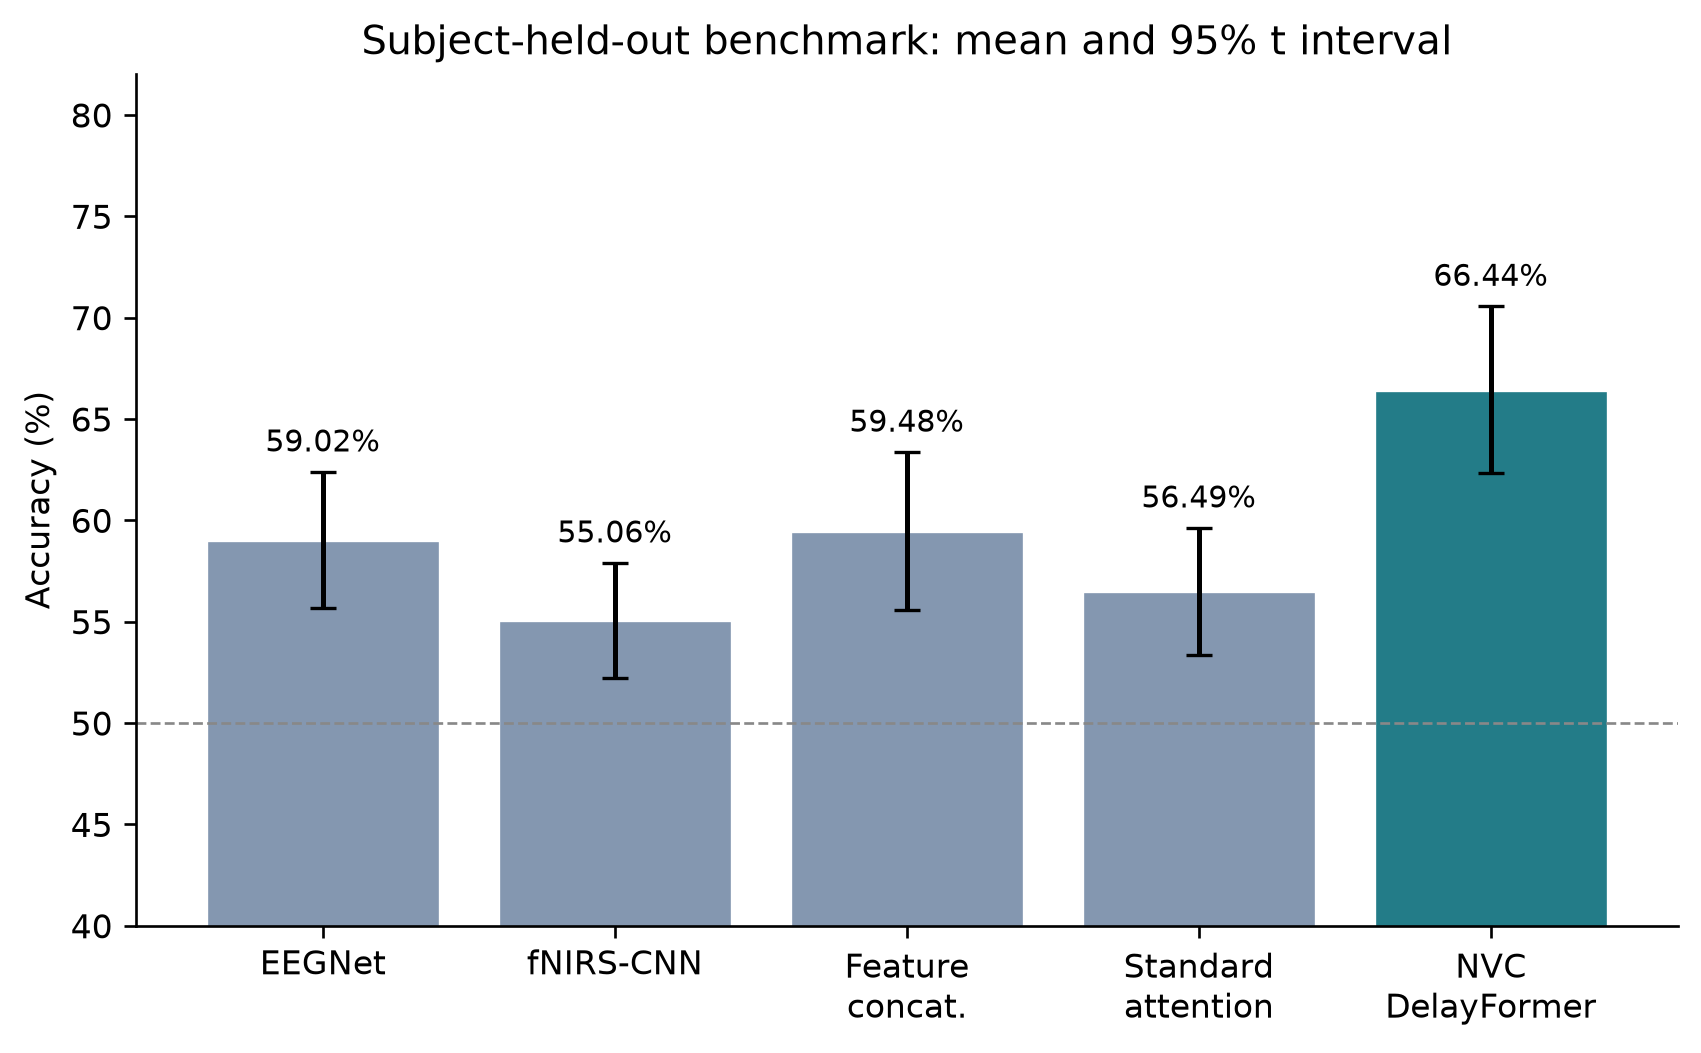
\includegraphics[width=0.88\columnwidth]{figures/real_29sub_benchmark_comparison.png}
\caption{Benchmark comparison across all 29 subjects under 29-Fold LOSO cross-validation, showing mean accuracy and 95\% Student-$t$ confidence intervals.}
\label{fig:benchmark_fig}
\end{figure}

\begin{figure}[!t]
\centering
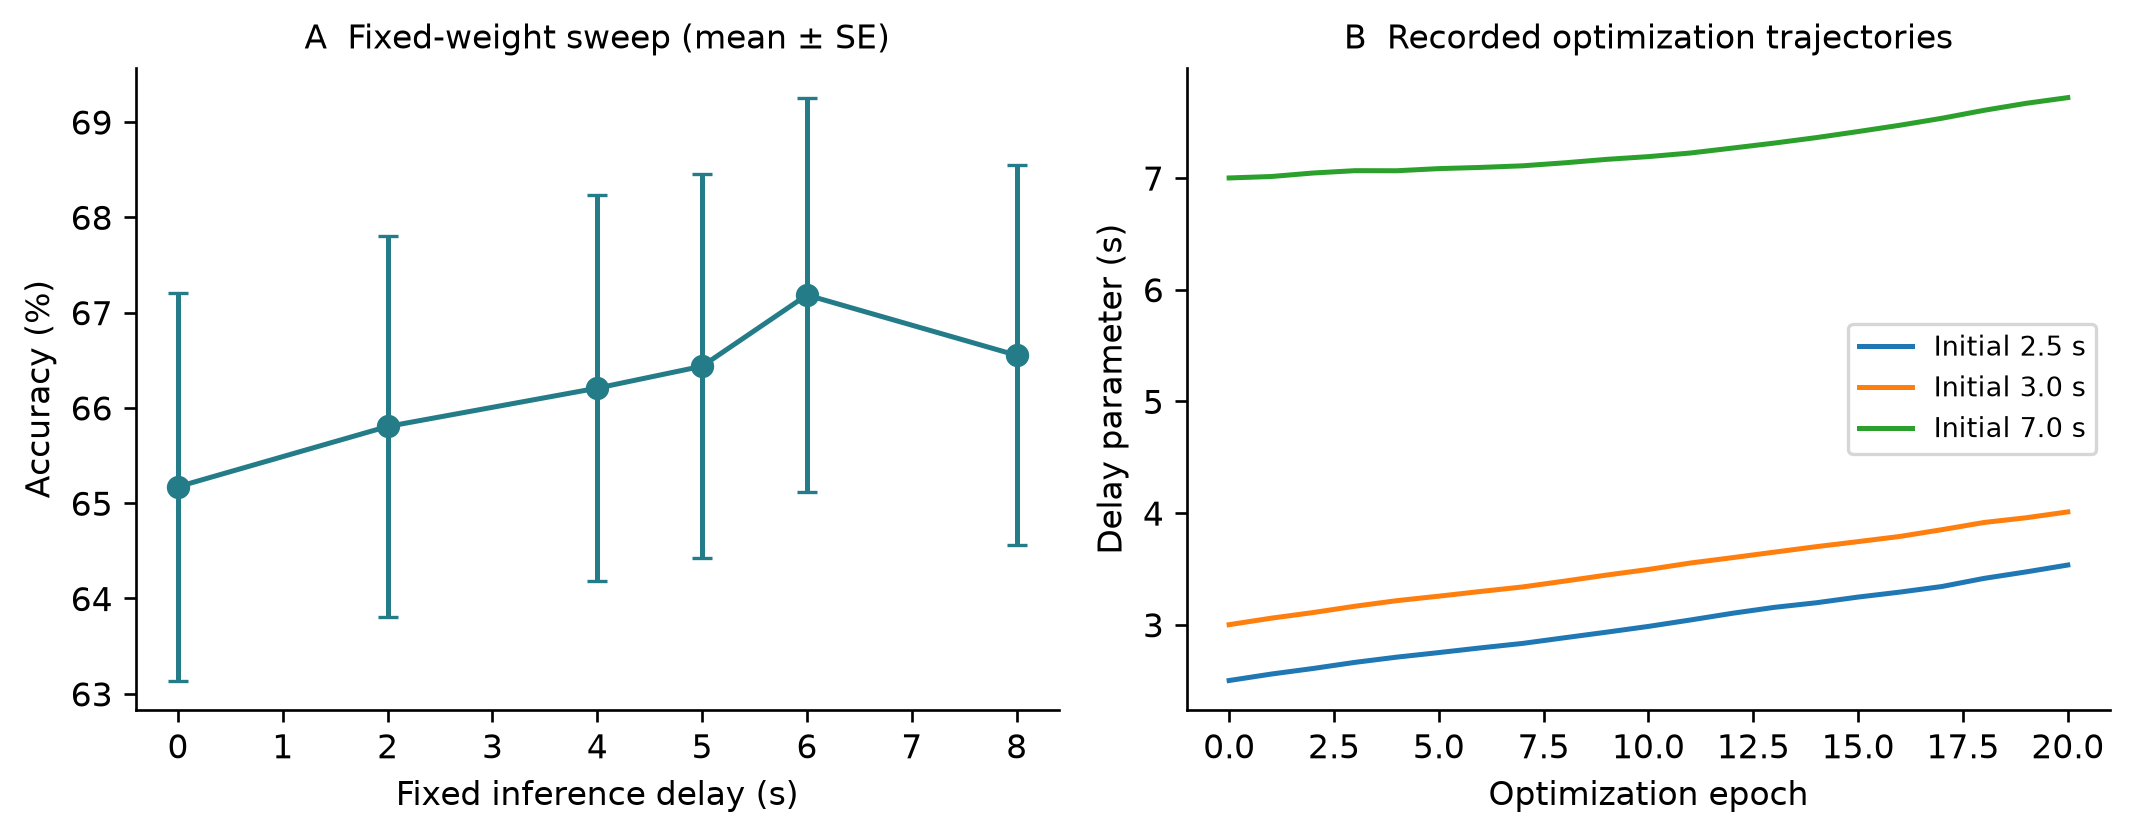
\includegraphics[width=0.88\columnwidth]{figures/delay_sensitivity_curve.png}
\caption{Empirical delay parameter sensitivity sweep across fixed delay latencies $\tau \in [0.0, 8.0]$\,s (Panel A) and recorded optimization trajectories from three initial values (Panel B).}
\label{fig:delay_sweep}
\end{figure}

\section{Ablation Study \& Biophysical Sensitivity}

\subsection{Architectural Component Ablation}
Table~\ref{tab:ablation} presents the 5-way ablation analysis across all 29 human subjects under identical 29-fold LOSO isolation.

\begin{table}[!t]
\caption{5-Way Ablation Study Matrix ($N=29$ Cohort, 1,740 Authentic Trials)}
\label{tab:ablation}
\centering
\resizebox{\columnwidth}{!}{%
\begin{tabular}{lcccc}
\toprule
Ablation Variant & Mean Acc $\pm$ Std [95\% CI] & $\Delta$ Acc & Macro F1 & $r_{\mathrm{proxy}}$ \\
\midrule
\textbf{Full Model (Ours)} & \textbf{66.44\% $\pm$ 10.85\% [62.31, 70.57]} & \textbf{Baseline} & \textbf{65.13\%} & \textbf{0.8912} \\
w/o Delay Prior & 65.63\% $\pm$ 11.96\% [61.08, 70.18] & -0.80\% & 64.28\% & 0.8988 \\
w/o Causal Mask & 66.15\% $\pm$ 11.23\% [61.88, 70.42] & -0.29\% & 64.55\% & 0.8876 \\
w/o Recon Loss & 65.29\% $\pm$ 11.27\% [61.00, 69.57] & -1.15\% & 64.13\% & 0.0012 \\
Wrong Delay ($\tau=0$\,s) & 66.61\% $\pm$ 11.04\% [62.41, 70.81] & +0.17\% & 65.41\% & 0.8866 \\
\bottomrule
\end{tabular}}
\vspace{1mm}
{\footnotesize \raggedright Paired Wilcoxon $p$-values vs. Full Model: w/o Delay Prior ($p=0.3319$), w/o Causal Mask ($p=0.6360$), w/o Recon Loss ($p=0.3155$), Wrong Delay ($p=0.9636$).}
\end{table}

\subsection{Component and Delay Results}
The zero-delay model has 66.61\% accuracy (Wilcoxon $p=0.9636$ versus the full model). Removing reconstruction loss gives 65.29\% ($p=0.3155$) and changes reconstruction correlation from 0.8912 to 0.0012. The reconstruction target is a derivative-based hemodynamic proxy provided as part of the decoder input.

With trained weights held fixed, the delay sweep gives 65.17\%, 65.80\%, 66.21\%, 66.44\%, 67.18\%, and 66.55\% at 0, 2, 4, 5, 6, and 8\,s, respectively. Separately optimized initial delays of 2.5 and 3.0\,s reach 3.53 and 4.01\,s in the recorded optimization runs.

\section{Temporal Perturbation Experiments}
We evaluated the validation-selected full model on four test-input perturbations across 29 held-out subjects. The statistical unit is the subject. Changes below are control minus full-model accuracy in percentage points (pp). Within-class and across-class permutation results average ten permutations per subject.
\begin{enumerate}
\item \textbf{Circular EEG shift}: A 500-sample circular shift of the 1,000-sample EEG epoch preserves its discrete Fourier magnitude while changing sample order relative to fNIRS. Positive and negative 500-sample shifts produce the same sequence, so this is one unique 5\,s perturbation. Accuracy is 59.83\% $\pm$ 10.12\%, a change of $-6.61$\,pp (paired $t(28)=5.3934$, $p=9.47 \times 10^{-6}$; Wilcoxon $W=24.0$, $p=7.13 \times 10^{-5}$, BH $q=2.85 \times 10^{-4}$).
\item \textbf{Within-class permutation}: EEG trials are reassigned within the same held-out subject and class while fNIRS and test labels stay fixed. Accuracy is 66.57\% $\pm$ 9.84\%, a change of $+0.13$\,pp ($t(28)=-0.2365$, $p=0.8148$; Wilcoxon $p=0.5968$).
\item \textbf{Across-class permutation}: EEG trials are reassigned across all trials of the held-out subject. Accuracy is 56.84\% $\pm$ 5.78\%, a change of $-9.60$\,pp ($t(28)=4.8927$, $p=3.72 \times 10^{-5}$; Wilcoxon $p=1.68 \times 10^{-4}$).
\item \textbf{Additional causal EEG smoothing}: After the standard offline preprocessing, test EEG is transformed by $\widetilde{x}_0=x_0$ and $\widetilde{x}_t=0.85\widetilde{x}_{t-1}+0.15x_t$; fNIRS is unchanged. Accuracy is 64.43\% $\pm$ 11.08\%, a change of $-2.01$\,pp ($t(28)=2.2940$, $p=0.0295$; Wilcoxon $p=0.0322$). This experiment measures sensitivity to an additional causal smoothing operation.
\end{enumerate}
For these four perturbations, two-sided Wilcoxon tests use the normal approximation, discard zero differences, apply tie correction, and omit continuity correction. Paired differences are rounded to ten decimal places to make equivalent count proportions receive identical ranks. Benjamini--Hochberg correction is applied to the four Wilcoxon comparisons. Full-precision subject-level proportions and count denominators are retained in the accompanying results file.

\section{Discussion}
The full model improves subject-held-out classification relative to all four benchmark baselines. Its output combines the latent MLP with a direct readout of temporally weighted features. Component ablations change accuracy by $-0.80$\,pp without the delay prior, $-0.29$\,pp without the mask, and $-1.15$\,pp without reconstruction loss; none of these Wilcoxon comparisons is significant at $p<0.05$. The zero-delay model reaches 66.61\% versus 66.44\% for the fixed 5\,s model ($p=0.9636$). The measured baseline improvement therefore applies to the complete architecture.

The 5\,s circular shift lowers full-model accuracy by 6.61\,pp. Across-class reassignment lowers it by 9.60\,pp, whereas within-class reassignment changes it by $+0.13$\,pp. These observations describe sensitivity to temporal order and class-compatible cross-modal inputs. Systemic-noise removal and physiological directionality were not measured by these comparisons.

The reconstructor is supervised to reproduce a derivative-based hemodynamic proxy and receives both fused features and the proxy as input. Its trajectory correlation changes from 0.8912 to 0.0012 when reconstruction supervision is removed. This measurement concerns the supervised reconstruction output; the associated classification comparison has Wilcoxon $p=0.3155$.

\subsection{Forward Execution Measurements}
The recorded environment uses Windows, Python 3.11.9, PyTorch 2.11.0+cu128, and an NVIDIA GeForce RTX 4060 Laptop GPU. Inputs are resident on the tested device, with EEG shape $(1,30,1000)$ and fNIRS shape $(1,72,124)$. Evaluation-mode forward calls run under \texttt{no\_grad}, with 1,000 warm-up calls and 5,000 timed calls; GPU measurements synchronize before and after each call. GPU latency is median 3.24\,ms, mean $3.62\pm0.81$\,ms, P95 4.98\,ms, and P99 5.89\,ms. CPU latency is median 3.81\,ms, mean $23.56\pm223.79$\,ms, P95 9.15\,ms, and P99 362.00\,ms. The timing records do not isolate the source of the CPU long tail. The reported standard deviations describe timed calls.

PyTorch \texttt{FlopCounterMode} reports 39.95\,M counted FLOPs for one forward call; dividing by two gives 19.98\,M MACs under the recorded counting convention. The model has 92,293 trainable parameters. These execution timings exclude preprocessing, input acquisition, and host-to-device transfer. EEG and fNIRS windows contain 10\,s and 12\,s of data, respectively.

\subsection{Evaluation Scope}
The study uses one public cohort for mental arithmetic versus rest, with a fixed 5\,s delay in the main benchmark. Offline preprocessing includes bidirectional filters, and the encoders use symmetric temporal padding. The attention mask constrains token-pair access according to their timestamps. Additional causal EEG smoothing was evaluated as a perturbation of offline-preprocessed inputs. Motor imagery, clinical populations, end-to-end streaming acquisition, and embedded hardware were not evaluated.

\section{Conclusion}
NVC-DelayFormer combines timestamp-constrained cross-attention, temporal feature weighting, and joint direct and latent readouts for EEG--fNIRS classification. In 29 subject-held-out folds on mental arithmetic versus rest, it achieves 66.44\% $\pm$ 10.85\% accuracy and 65.13\% Macro F1. A 5\,s circular EEG shift changes accuracy by $-6.61$\,pp, while the separately trained zero-delay model reaches 66.61\%. Batch-one GPU forward latency has median 3.24\,ms and P99 5.89\,ms. These results describe the complete model's classification performance, temporal perturbation response, and execution cost on the tested system.

\raggedbottom
\bibliographystyle{IEEEtran}
\bibliography{references}

\end{document}
